\documentclass[journal, a4paper]{IEEEtran}

% some very useful LaTeX packages include:

%\usepackage{cite}      % Written by Donald Arseneau
                        % V1.6 and later of IEEEtran pre-defines the format
                        % of the cite.sty package \cite{} output to follow
                        % that of IEEE. Loading the cite package will
                        % result in citation numbers being automatically
                        % sorted and properly "ranged". i.e.,
                        % [1], [9], [2], [7], [5], [6]
                        % (without using cite.sty)
                        % will become:
                        % [1], [2], [5]--[7], [9] (using cite.sty)
                        % cite.sty's \cite will automatically add leading
                        % space, if needed. Use cite.sty's noadjust option
                        % (cite.sty V3.8 and later) if you want to turn this
                        % off. cite.sty is already installed on most LaTeX
                        % systems. The latest version can be obtained at:
                        % http://www.ctan.org/tex-archive/macros/latex/contrib/supported/cite/

\usepackage{graphicx}   % Written by David Carlisle and Sebastian Rahtz
                        % Required if you want graphics, photos, etc.
                        % graphicx.sty is already installed on most LaTeX
                        % systems. The latest version and documentation can
                        % be obtained at:
                        % http://www.ctan.org/tex-archive/macros/latex/required/graphics/
                        % Another good source of documentation is "Using
                        % Imported Graphics in LaTeX2e" by Keith Reckdahl
                        % which can be found as esplatex.ps and epslatex.pdf
                        % at: http://www.ctan.org/tex-archive/info/

%\usepackage{psfrag}    % Written by Craig Barratt, Michael C. Grant,
                        % and David Carlisle
                        % This package allows you to substitute LaTeX
                        % commands for text in imported EPS graphic files.
                        % In this way, LaTeX symbols can be placed into
                        % graphics that have been generated by other
                        % applications. You must use latex->dvips->ps2pdf
                        % workflow (not direct pdf output from pdflatex) if
                        % you wish to use this capability because it works
                        % via some PostScript tricks. Alternatively, the
                        % graphics could be processed as separate files via
                        % psfrag and dvips, then converted to PDF for
                        % inclusion in the main file which uses pdflatex.
                        % Docs are in "The PSfrag System" by Michael C. Grant
                        % and David Carlisle. There is also some information
                        % about using psfrag in "Using Imported Graphics in
                        % LaTeX2e" by Keith Reckdahl which documents the
                        % graphicx package (see above). The psfrag package
                        % and documentation can be obtained at:
                        % http://www.ctan.org/tex-archive/macros/latex/contrib/supported/psfrag/

%\usepackage{subfigure} % Written by Steven Douglas Cochran
                        % This package makes it easy to put subfigures
                        % in your figures. i.e., "figure 1a and 1b"
                        % Docs are in "Using Imported Graphics in LaTeX2e"
                        % by Keith Reckdahl which also documents the graphicx
                        % package (see above). subfigure.sty is already
                        % installed on most LaTeX systems. The latest version
                        % and documentation can be obtained at:
                        % http://www.ctan.org/tex-archive/macros/latex/contrib/supported/subfigure/

\usepackage{url}        % Written by Donald Arseneau
                        % Provides better support for handling and breaking
                        % URLs. url.sty is already installed on most LaTeX
                        % systems. The latest version can be obtained at:
                        % http://www.ctan.org/tex-archive/macros/latex/contrib/other/misc/
                        % Read the url.sty source comments for usage information.

%\usepackage{stfloats}  % Written by Sigitas Tolusis
                        % Gives LaTeX2e the ability to do double column
                        % floats at the bottom of the page as well as the top.
                        % (e.g., "\begin{figure*}[!b]" is not normally
                        % possible in LaTeX2e). This is an invasive package
                        % which rewrites many portions of the LaTeX2e output
                        % routines. It may not work with other packages that
                        % modify the LaTeX2e output routine and/or with other
                        % versions of LaTeX. The latest version and
                        % documentation can be obtained at:
                        % http://www.ctan.org/tex-archive/macros/latex/contrib/supported/sttools/
                        % Documentation is contained in the stfloats.sty
                        % comments as well as in the presfull.pdf file.
                        % Do not use the stfloats baselinefloat ability as
                        % IEEE does not allow \baselineskip to stretch.
                        % Authors submitting work to the IEEE should note
                        % that IEEE rarely uses double column equations and
                        % that authors should try to avoid such use.
                        % Do not be tempted to use the cuted.sty or
                        % midfloat.sty package (by the same author) as IEEE
                        % does not format its papers in such ways.

\usepackage{amsmath}    % From the American Mathematical Society
                        % A popular package that provides many helpful commands
                        % for dealing with mathematics. Note that the AMSmath
                        % package sets \interdisplaylinepenalty to 10000 thus
                        % preventing page breaks from occurring within multiline
                        % equations. Use:
%\interdisplaylinepenalty=2500
                        % after loading amsmath to restore such page breaks
                        % as IEEEtran.cls normally does. amsmath.sty is already
                        % installed on most LaTeX systems. The latest version
                        % and documentation can be obtained at:
                        % http://www.ctan.org/tex-archive/macros/latex/required/amslatex/math/



% Other popular packages for formatting tables and equations include:

%\usepackage{array}
% Frank Mittelbach's and David Carlisle's array.sty which improves the
% LaTeX2e array and tabular environments to provide better appearances and
% additional user controls. array.sty is already installed on most systems.
% The latest version and documentation can be obtained at:
% http://www.ctan.org/tex-archive/macros/latex/required/tools/

% V1.6 of IEEEtran contains the IEEEeqnarray family of commands that can
% be used to generate multiline equations as well as matrices, tables, etc.

% Also of notable interest:
% Scott Pakin's eqparbox package for creating (automatically sized) equal
% width boxes. Available:
% http://www.ctan.org/tex-archive/macros/latex/contrib/supported/eqparbox/

% *** Do not adjust lengths that control margins, column widths, etc. ***
% *** Do not use packages that alter fonts (such as pslatex).         ***
% There should be no need to do such things with IEEEtran.cls V1.6 and later.


% Your document starts here!
\begin{document}
\begin{titlepage}

\newcommand{\HRule}{\rule{\linewidth}{0.5mm}} % Defines a new command for the horizontal lines, change thickness here

\center % Center everything on the page
 %----------------------------------------------------------------------------------------
%	LOGO SECTION
%----------------------------------------------------------------------------------------

~\\[1cm]

\includegraphics{SCUT.png}\\[2cm] % Include a department/university logo - this will require the graphicx package

%----------------------------------------------------------------------------------------
%	TITLE SECTION
%----------------------------------------------------------------------------------------

\HRule \\[1cm]
{ \huge \bfseries The Experiment Report of \textit{Machine Learning} }\\[0.6cm] % Title of your document
\HRule \\[2cm]
%----------------------------------------------------------------------------------------
%	HEADING SECTIONS
%----------------------------------------------------------------------------------------


\textsc{\LARGE \textbf{School:} School of Software Engineering}\\[1cm]
\textsc{\LARGE \textbf{Subject:} Software Engineering}\\[2cm] 

 
%----------------------------------------------------------------------------------------
%	AUTHOR SECTION
%----------------------------------------------------------------------------------------

\begin{minipage}{0.4\textwidth}
\begin{flushleft} \large
\emph{Author:}\\
Biquan Wang, Li Li, and Yuchen Li% Your name
\end{flushleft}
\end{minipage}
~
\begin{minipage}{0.4\textwidth}
\begin{flushright} \large
\emph{Supervisor:} \\
Qingyao Wu % Supervisor's Name
\end{flushright}
\end{minipage}\\[2cm]
~
\begin{minipage}{0.4\textwidth}
\begin{flushleft} \large
\emph{Student ID:}\\
201821038853, 201820137894, and 201821038741
\end{flushleft}
\end{minipage}
~
\begin{minipage}{0.4\textwidth}
\begin{flushright} \large
\emph{Grade:} \\
Graduate
\end{flushright}
\end{minipage}\\[2cm]

% If you don't want a supervisor, uncomment the two lines below and remove the section above
%\Large \emph{Author:}\\
%John \textsc{Smith}\\[3cm] % Your name

%----------------------------------------------------------------------------------------
%	DATE SECTION
%----------------------------------------------------------------------------------------

{\large \today}\\[2cm] % Date, change the \today to a set date if you want to be precise

 
%----------------------------------------------------------------------------------------

\vfill % Fill the rest of the page with whitespace

\end{titlepage}

% Define document title and author
	\title{Recommender System Based on Matrix Factorization}
	\maketitle

% Write abstract here
\begin{abstract}
Matrix factorization can be used to discover latent features underlying the interactions between two or more different kinds of entities. So, one obvious application is to predict ratings in recommender system. In tihs paper, we use matrix factorization with stochastic gradient descent to gnerate a predict matrix from  discrete data. For futher understanding, we try to show the result with different learn rate and different latent feature number $K$, and try to find the impact of these two prameters. 
\end{abstract}

% Each section begins with a \section{title} command
\section{Introduction}
	% \PARstart{}{} creates a tall first letter for this first paragraph
\PARstart{M}{atrix} factorization is one of the most popular methods for collaborative filtering recommendation, and stochastic gradient descent is the most common optimize way for black-box optimize problem. RMSE(Root mean Square Error)is a commonly used regression evaluation standard.

This paper aim to show the process of matrix factorization, we try two show the result with different learn rate and different latent feature number $K$, and try to find the impact of these two prameters.

% Main Part
\section{Methods and Theory}
In this part, we try to explain the process of matrix decomposition from idea to implementation. At the end, we explan the loss function and the update function of the factor matrix with stochastic gradient descent.

Example for this data set, we have a set $U$ of users, and a set of $D$ of movies. $\boldsymbol{R}$ is the rating matrix size $|U|\times|D|$. And assume that we want to find $K$ latent features. So, what we should do is to find two matrix: $\boldsymbol{P}$($|U|\times K$) and $\boldsymbol{Q}$($|D|\times K$), such that their product approximates $\boldsymbol{R}$:
\begin{displaymath}
\boldsymbol{R}\approx \boldsymbol{P}\times \boldsymbol{Q}^T=\hat{\boldsymbol{R}}
\end{displaymath} 

In this way, $\boldsymbol{P}$ represent the strength of the associations between a user and the latent features, at the same times, $\boldsymbol{Q}$ represent the strength of the associations between a movie and the latent features.
\begin{displaymath}
\hat{r}_{ij} = p_i^Tq_j=\sum_{k=1}^kp_{ik}q_{kj}
\end{displaymath}
In this experiment, We use gradient descent to get suitable $\boldsymbol{P}$ and $\boldsymbol{Q}$ : initialize the two matrices with some value, calculate how "different" their product $\hat{R}$ to $R$, and try to minimize the difference interactively. 

The difference here we called loss between the predict rating and real rating can use following function to calculate, we use squared error because the predict rating can be either higher or lower than real rating:
\begin{displaymath}
loss_{ij}^2=(r_{ij}-\hat{r}_{ij})^2=(r_{ij}-\sum_{k=1}^Kp_{ik}q_{kj})^2
\end{displaymath}
Add regularization to avoid overfitting:
\begin{eqnarray}
loss_{ij}^2=(r_{ij}-\sum_{k=1}^Kp_{ik}q_{kj})^2+\frac{\beta}{2}\sum_{k=1}^K(||\boldsymbol{P}||^2+||\boldsymbol{Q}||^2)
\end{eqnarray}
In gradient descent, we need to know the gradient of $p_{ik}$ and $q_{kj}$, so, we differentiate the above function with respect to these two variables separately:
\begin{displaymath}
\frac{\partial loss_{ij}^2}{\partial p_{ik}}=2loss_{ij}q_{kj}-\beta p_{ik}
\end{displaymath}
\begin{displaymath}
\frac{\partial loss_{ij}^2}{\partial q_{kj}}=2loss_{ij}p_{ik}-\beta q_{kj}
\end{displaymath}
So, the update function with learn rate $\eta$ is:
\begin{eqnarray}
p'_{ik}=p_{ik}+\frac{\partial loss_{ij}^2}{\partial p_{ik}}=p_{ik}+\eta(2loss_{ij}q_{kj}-\beta p_{ik})
\end{eqnarray}
\begin{eqnarray}
q'_{kj}=q_{kj}+\frac{\partial loss_{ij}^2}{\partial q_{kj}}=q_{kj}+\eta(2loss_{ij}p_{ik}-\beta q_{kj})
\end{eqnarray}
RMSE:
\begin{eqnarray}
RMSE=\sqrt{\frac{1}{n}\sum_{i=1}^n(y_i-\hat{y_i})^2}
\end{eqnarray}


\section{Experiments}
\subsection{Dataset}
Utilizing MovieLens-100k dataset. u.data -- Consisting 10,000 comments from 943 users out of 1682 movies. At least, each user comment 20 videos. Users and movies are numbered consecutively from number 1 respectively. The data is sorted randomly

\begin{table}[!htb]
	\begin{center}
	\caption{Snapshot of input data}
	\label{tab:closed form}
	\begin{tabular}{|c|c|c|c|}
		\hline
		userid &  movieid & Rating & timestamp\\
		\hline
		196 & 242 & 3 &  881250949\\
		\hline
		ratings[n,0] & ratings[n,1] & ratings[n,2] & ratings[n,3] \\
		\hline
		12 & 203 & 3 &  879959583\\
		\hline
	\end{tabular}
	\end{center}
\end{table}

\subsection{Experiments steps}
The steps of our matrix factorization are as the following:
\begin{itemize}
\item[1.] Use loadtxt function in numpy library to load the MovieLens-100k and divided into train set and valid set.
\item[2.] Populate the original scoring matrix $R$ against the row data, and fill 0 for null values.
\item[3.]Initialize the user factor matrix $P$ and the item(Movie) factor matrix $Q$ and $K$ is the number of latent features.
\item[4.] Get a mini-batch data from train set randomly.
\item[5.] Update factor matrix $P$ with function (2), and update factor matrix $Q$ with fuction (3).
\item[6.] Calculate the loss of validation set with function (1).
\item[7.] Repeate setp 4-6 for n times, and return the losses of validation set.
\end{itemize}

\subsection{Experiments Results}
In this experiment we try to compare the impact of learn rate and latent factor $K$, so, the other hyper parameters is same: batch-size=10000, epoch=200, plenty=0.02.

Figure 1 is the result of $K=2$, and different learn rate, we can find out that, with the increase of learn rate, the loss decrease faster. We try two use a large enough learn rate such as 0.02, 0.2 etc, but the program will overflow, so we can not show the overfitting result. 
Figure 2 is the result of $K=3$, and different learn rate.

From Figure 1 and 2, we chose learn rate 0.005 as a local best learn rate and compare the result with different $K$. From figure 3, we can see, the loss begin with smaller number, with increase of latent factor $K$.
\begin{figure}[!htb]
	\begin{center}
	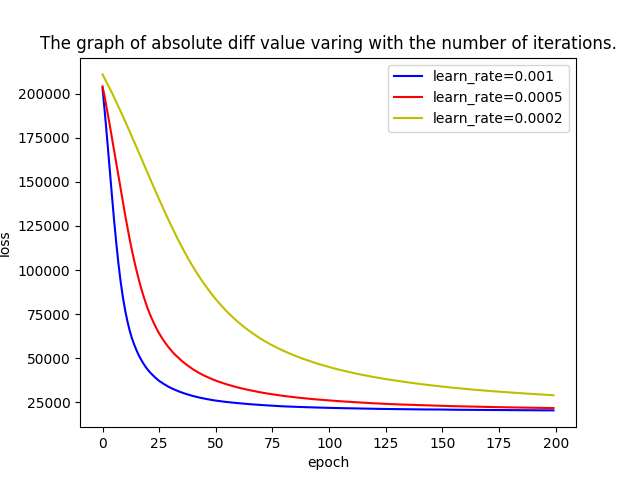
\includegraphics[width=\columnwidth]{mf_k2}
	\caption{Losses of different learn rate with k=2}
	\label{fig:mf_k2}
	\end{center}
\end{figure}

\begin{figure}[!htb]
	\begin{center}
	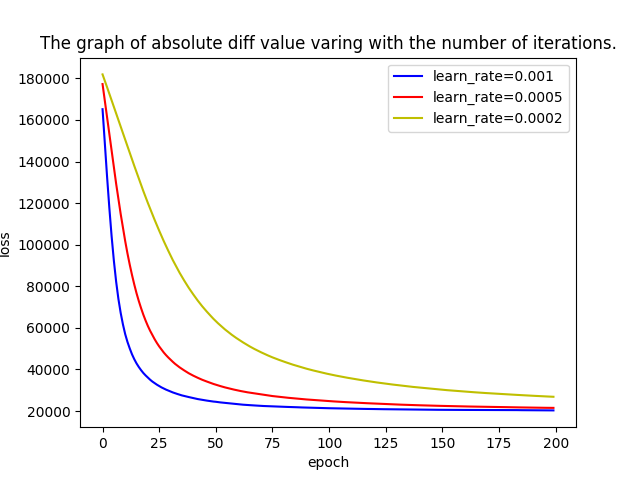
\includegraphics[width=\columnwidth]{mf_k3}
	\caption{Losses of different learn rate with k=3}
	\label{fig:mf_k3}
	\end{center}
\end{figure}

\begin{figure}[!htb]
	\begin{center}
	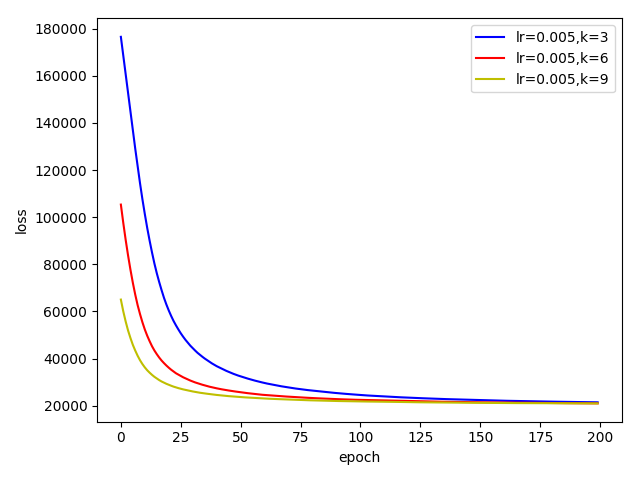
\includegraphics[width=\columnwidth]{mf_k_compare}
	\caption{Losses of different $K$ learn rate 0.005}
	\label{fig:mf_k_compare}
	\end{center}
\end{figure}

\begin{figure}[!htb]
	\begin{center}
	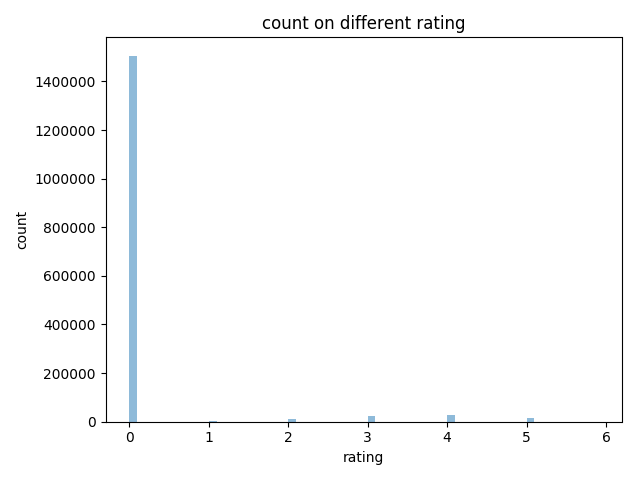
\includegraphics[width=\columnwidth]{mf_cr_0}
	\caption{Rating distribution with 0}
	\label{fig:mf_cr_0}
	\end{center}
\end{figure}

\begin{figure}[!htb]
	\begin{center}
	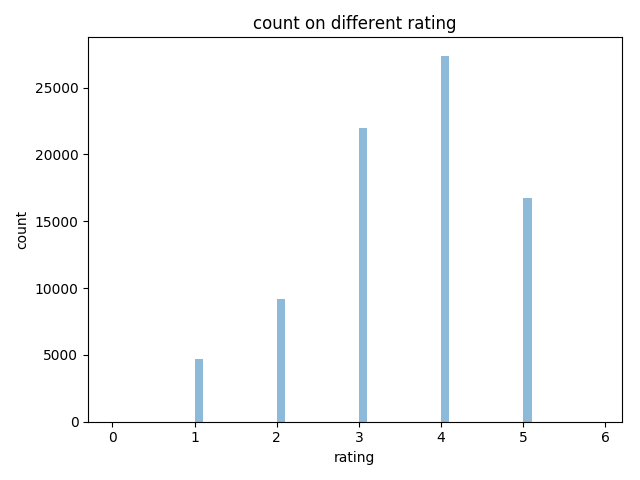
\includegraphics[width=\columnwidth]{mf_cr}
	\caption{Rating distribution without 0}
	\label{fig:mf_cr}
	\end{center}
\end{figure}

\begin{figure}[!htb]
	\begin{center}
	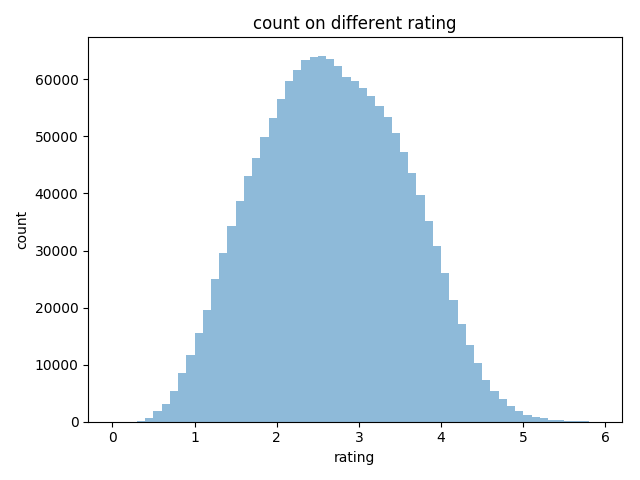
\includegraphics[width=\columnwidth]{mf_cr_k3}
	\caption{Rating distribution after MF with K=3}
	\label{fig:mf_cr_k3}
	\end{center}
\end{figure}

\begin{figure}[!htb]
	\begin{center}
	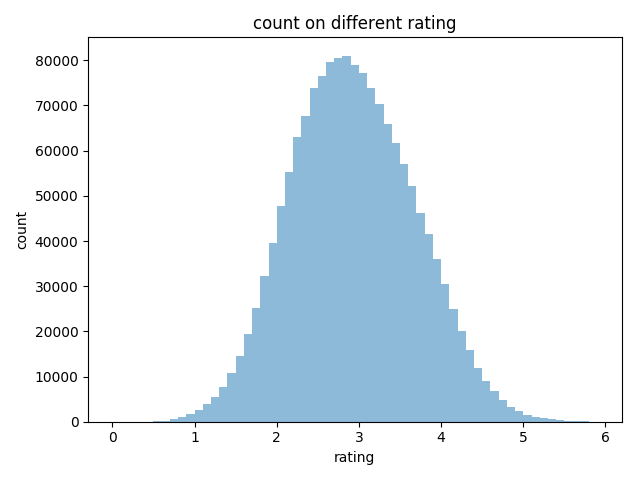
\includegraphics[width=\columnwidth]{mf_cr_k6}
	\caption{Rating distribution after MF with K=6}
	\label{fig:mf_cr_k6}
	\end{center}
\end{figure}

\begin{figure}[!htb]
	\begin{center}
	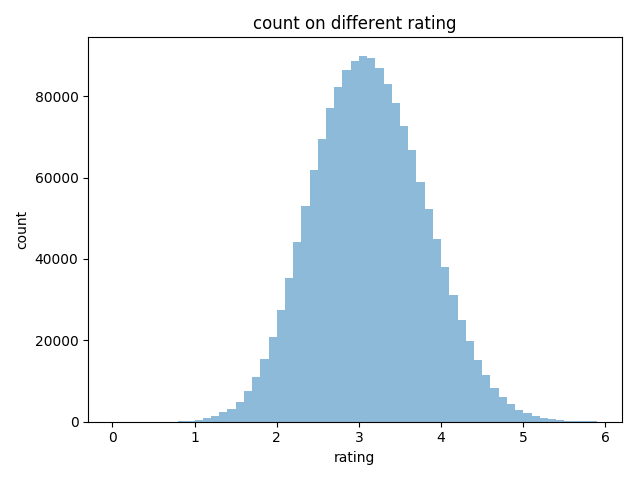
\includegraphics[width=\columnwidth]{mf_cr_k9}
	\caption{Rating distribution after MF with K=9}
	\label{fig:mf_cr_k9}
	\end{center}
\end{figure}
\begin{figure}[!htb]
	\begin{center}
	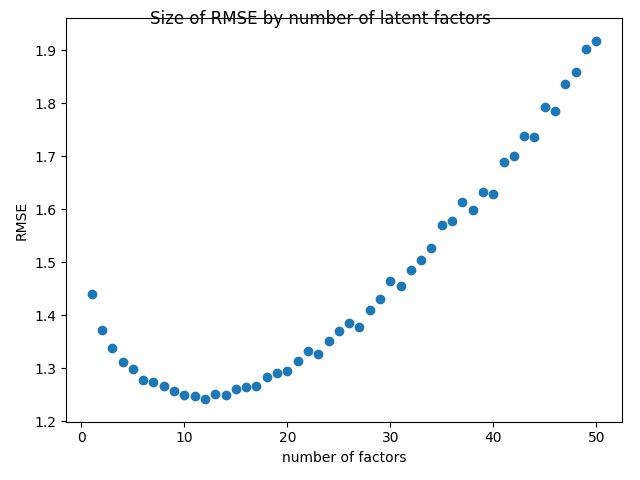
\includegraphics[width=\columnwidth]{mf_rmse}
	\caption{RMSE with different latent feature number $K$}
	\label{fig:mf_rmse}
	\end{center}
\end{figure}



Figure 4 and 5 shows the distribution of rating before algorithm, and figure 4 is the input matrix, witch contins 0(no rating).

Figure 6,7,8 shows the distribution of rating of predict matrix with $K$=3,6,9, from these pictures we can see that, there is no 0 rating, and all data tends to be normally distributed.

For further compare the impact of different latent feature, Figure 9 shows the RMSE value of predict matrix with different value of $K$. We can find out when $K$=12 the RMSE value is smallest.
\section{Conclusion}
	In tihs paper, we use matrix factorization with SGD to gnerate a predict matrix from  discrete data. For easy to understanding, we compare the result with different learn rate and different latent feature number $K$, and try to find the impact of these two prameters. We just finish the key step of a whole recommender system because of the time limitation, and we will compare other algorithm such as collaborative filtering, etc.



% Your document ends here!
\end{document}